



%%=============================================================================
\section{Application: L'Hospital's Rule}
\index{L'Hospital's rule}

\paragraph{}
Some singularities are easy to diagnose.  Consider the function 
$\frac{\cos x}{x}$ at the point $x = 0$.  The function evaluates to 
$\frac{1}{0}$ and is thus discontinuous at that point.  Since the numerator
and denominator are continuous functions and the denominator vanishes while
the numerator does not, the left and right limits as $x \to 0$ do not 
exist.  Thus the function has an infinite discontinuity at the point
$x = 0$.  

\begin{figure}[h!]
%\begin{tabular}{cc}
\begin{minipage}{\textwidth}
\begin{center}
%\vspace{1.0 cm}
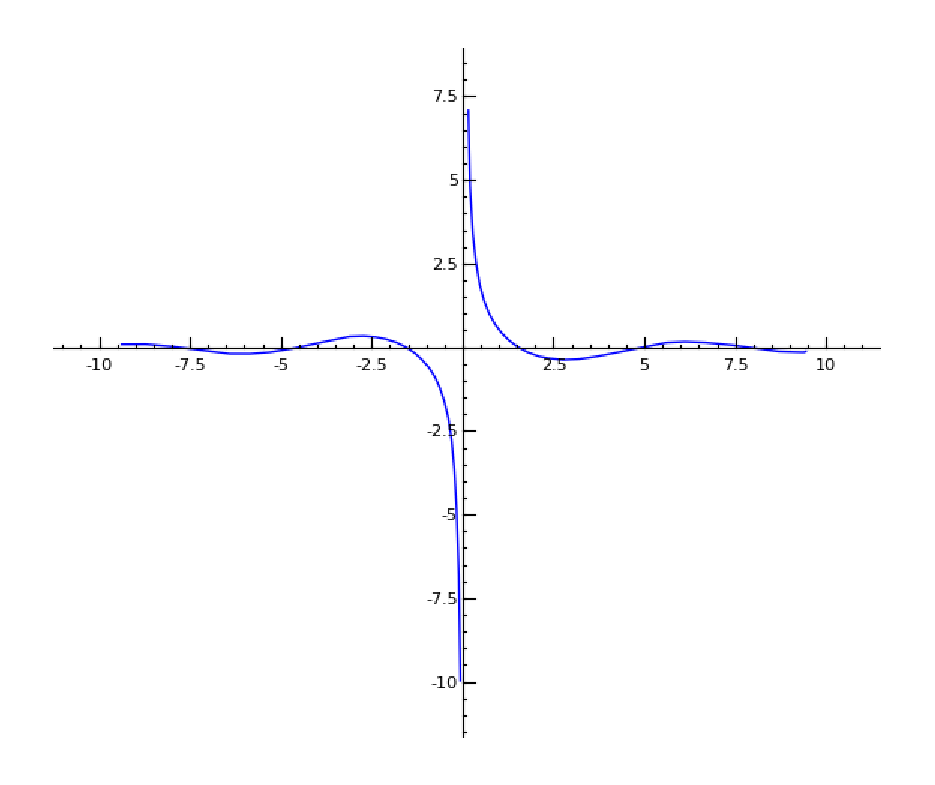
\includegraphics[height=5cm,width=10cm]{cosoverx.eps}
\end{center}
\end{minipage}
\caption{$\frac{\cos(x)}{x}$.}
\label{fig:cosoverx}
\end{figure}

\noindent
More generally, a function which is composed of continuous
functions and evaluates to $\frac{a}{0}$ at a point where $a \neq 0$ must
have an infinite discontinuity there.

\paragraph{}
Other singularities require more analysis to diagnose.  Consider the 
functions $\frac{\sin x}{x}$, $\frac{\sin x}{|x|}$ and 
$\frac{\sin x}{1 - \cos x}$ at the point $x = 0$.  All three functions
evaluate to $\frac{0}{0}$ at that point, but have different kinds
of singularities.  The first has a removable discontinuity, the second has
a finite discontinuity and the third has an infinite discontinuity.
See Figure~\ref{disc3}.

\begin{figure}[h!]
%\begin{tabular}{cc}
\begin{minipage}{\textwidth}
\begin{center}
%\vspace{1.0 cm}
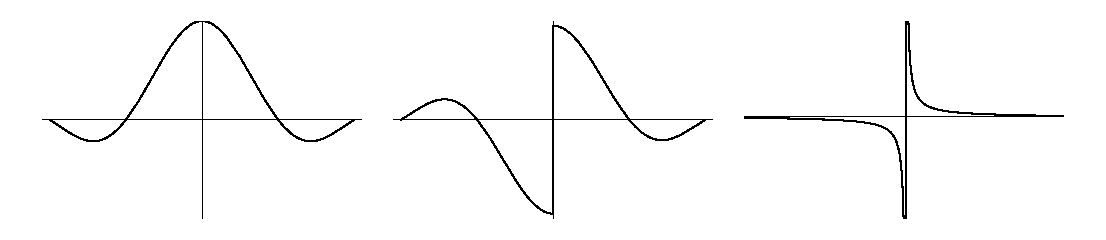
\includegraphics[height=4cm,width=10cm]{disc3.eps}
\end{center}
\end{minipage}
\caption{The functions $\frac{\sin x}{x}$, $\frac{\sin x}{|x|}$ and
    $\frac{\sin x}{1 - \cos x}$.}
\label{fig:disc3}
\label{disc3}
\end{figure}

An expression that evaluates to $\frac{0}{0}$, $\frac{\infty}{\infty}$,
$0 \cdot \infty$, $\infty - \infty$, $1^\infty$, $0^0$ or $\infty^0$
is called an \textit{indeterminate}.  A function $f(x)$ which is indeterminate
at the point $x = \xi$ is singular at that point.  The singularity may be a 
removable discontinuity, a finite discontinuity or an infinite discontinuity
depending on the behavior of the function around that point.  If
$\lim_{x \to \xi} f(x)$ exists, then the function has a removable 
discontinuity.  If the limit does not exist, but the left and right limits 
do exist, then the function has a finite discontinuity.  If either the
left or right limit does not exist then the function has an infinite
discontinuity.





{\bf L'Hospital's Rule.}
Let $f(x)$ and $g(x)$ be differentiable and $f(\xi) = g(\xi) = 0$.  
Further, let $g(x)$ be nonzero in a deleted neighborhood of $x= \xi$, 
($g(x) \neq 0$ for $x \in 0 < |x - \xi| < \delta$).  Then
\[
\lim_{x \to \xi} \frac{f(x)}{g(x)} = \lim_{x \to \xi} \frac{f'(x)}{g'(x)}.
\]
To prove this, we note that $f(\xi) = g(\xi) = 0$ and apply the generalized
theorem of the mean.  Note that
\[
\frac{f(x)}{g(x)} = \frac{f(x) - f(\xi)}{g(x) - g(\xi)}
= \frac{f'(\psi)}{g'(\psi)}
\]
for some $\psi$ between $\xi$ and $x$.  Thus
\[
\lim_{x \to \xi} \frac{f(x)}{g(x)} 
= \lim_{\psi \to \xi} \frac{f'(\psi)}{g'(\psi)}
= \lim_{x \to \xi} \frac{f'(x)}{g'(x)}
\]
provided that the limits exist.

L'Hospital's Rule is also applicable when both functions tend to infinity
instead of zero or when the limit point, $\xi$, is at infinity.  It 
is also valid for one-sided limits.


L'Hospital's rule is directly applicable to the indeterminate forms
$\frac{0}{0}$ and $\frac{\infty}{\infty}$.


\begin{example}
{\rm
  Consider the three functions $\frac{\sin x}{x}$, $\frac{\sin x}{|x|}$ and
  $\frac{\sin x}{1 - \cos x}$ at the point $x = 0$.
  \[
  \lim_{x \to 0} \frac{\sin x}{x}
  = \lim_{x \to 0} \frac{\cos x}{1} 
  = 1
  \]
  Thus $\frac{\sin x}{x}$ has a removable discontinuity at $x = 0$.
  \[
  \lim_{x \to 0^+} \frac{\sin x}{|x|}
  = \lim_{x \to 0^+} \frac{\sin x}{x} = 1
  \]
  \[
  \lim_{x \to 0^-} \frac{\sin x}{|x|}
  = \lim_{x \to 0^-} \frac{\sin x}{-x} = -1
  \]
  Thus $\frac{\sin x}{|x|}$ has a finite discontinuity at $x = 0$.
  \[
  \lim_{x \to 0} \frac{\sin x}{1 - \cos x}
  = \lim_{x \to 0} \frac{\cos x}{\sin x}
  = \frac{1}{0} = \infty
  \]
  Thus $\frac{\sin x}{1 - \cos x}$ has an infinite discontinuity at $x = 0$.
}
\end{example}



\begin{example}
{\rm
We use \sage to compute 
$\lim_{x\rightarrow 0}
\frac{\cos(x)-1}{x^2}$.

\vskip .1in

\begin{Verbatim}[fontsize=\scriptsize,fontfamily=courier,fontshape=tt,frame=single,label=\sage]

sage: limit((cos(x)-1)/x^2,x=0)
-1/2
sage: limit((-sin(x))/(2*x),x=0)
-1/2
sage: limit((-cos(x))/(2),x=0)
-1/2

\end{Verbatim}

\vskip .1in
\noindent
This verifies 

\[
\lim_{x\rightarrow 0}\frac{\cos(x)-1}{x^2}
=\lim_{x\rightarrow 0}\frac{-\sin(x)}{2x}
=\lim_{x\rightarrow 0}\frac{-\cos(x)}{2}=-1/2.
\]
}
\end{example}



\begin{example}
{\rm
  Let $a$ and $d$ be nonzero.
  \begin{align*}
    \lim_{x \to \infty} \frac{a x^2 + b x + c}{d x^2 + e x + f}
    &= \lim_{x \to \infty} \frac{2 a x + b}{2 d x + e} \\
    &= \lim_{x \to \infty} \frac{2 a}{2 d} \\
    &= \frac{a}{d}
  \end{align*}
}
\end{example}





\begin{example}
{\rm
Consider
  \[
  \lim_{x \to 0} \frac{\cos x - 1}{x \sin x}.
  \]
  This limit is an indeterminate of the form $\frac{0}{0}$.  Applying
  L'Hospital's rule we see that limit is equal to
  \[
  \lim_{x \to 0} \frac{-\sin x}{x \cos x + \sin x}.
  \]
  This limit is again an indeterminate of the form $\frac{0}{0}$.  We apply
  L'Hospital's rule again.
  \[
  \lim_{x \to 0} \frac{- \cos x}{ - x \sin x + 2 \cos x } = - \frac{1}{2}
  \]
  Thus the value of the original limit is $- \frac{1}{2}$.  We could also
  obtain this result by expanding the functions in Taylor series.
  \begin{align*}
    \lim_{x \to 0} \frac{\cos x - 1}{x \sin x}
    &= \lim_{x \to 0} \frac{\left( 1 - \frac{x^2}{2} + \frac{x^4}{24} 
        - \cdots \right) - 1 }{ x \left( x - \frac{x^3}{6} 
        + \frac{x^5}{120} - \cdots \right)} \\
    &= \lim_{x \to 0} \frac{- \frac{x^2}{2} + \frac{x^4}{24} - \cdots }
    { x^2 - \frac{x^4}{6} + \frac{x^6}{120} - \cdots } \\
    &= \lim_{x \to 0} \frac{- \frac{1}{2} + \frac{x^2}{24} - \cdots }
    { 1 - \frac{x^2}{6} + \frac{x^4}{120} - \cdots } \\
    &= - \frac{1}{2}
  \end{align*}
}
\end{example}




We can apply L'Hospital's Rule to the indeterminate forms $0 \cdot \infty$
and $\infty - \infty$ by rewriting the expression in a different form, 
(perhaps putting the expression over a common denominator).  If at first
you don't succeed, try, try again.  You may have to apply L'Hospital's 
rule several times to evaluate a limit.


\begin{example}
  \begin{align*}
    \lim_{x \to 0} \left( \cot x - \frac{1}{x} \right)
    &= \lim_{x \to 0} \frac{x \cos x - \sin x}{x \sin x} \\
    &= \lim_{x \to 0} \frac{\cos x - x \sin x - \cos x}
    {\sin x + x \cos x} \\
    &= \lim_{x \to 0} \frac{- x \sin x } {\sin x + x \cos x} \\
    &= \lim_{x \to 0} \frac{- x \cos x - \sin x } 
    {\cos x + \cos x - x \sin x } \\
    &= 0
  \end{align*}
\end{example}


You can apply L'Hospital's rule to the indeterminate forms $1^\infty$, 
$0^0$ or $\infty^0$ by taking the logarithm of the expression.


\begin{example}
{\rm
  Consider the limit,
  \[
  \lim_{x \to 0} x^x,
  \]
  which gives us the indeterminate form $0^0$.
  The logarithm of the expression is
  \[
  \ln( x^x ) = x \ln x.
  \]
  As $x \to 0$ we now have the indeterminate form $0 \cdot \infty$.  By 
  rewriting the expression, we can apply L'Hospital's rule.
  \begin{align*}
    \lim_{x \to 0} \frac{\ln x}{1/x}
    &= \lim_{x \to 0} \frac{1/x}{-1/x^2} \\
    &= \lim_{x \to 0} (-x) \\
    &= 0
  \end{align*}
  Thus the original limit is
  \[
  \lim_{x \to 0} x^x = e^0 = 1.
  \]
}
\end{example}

\section{Exercises}
Evaluate the following limits.

\begin{enumerate}
\item
%1.
  \renewcommand{\theenumi}{\alph{enumi}}
  \begin{enumerate}
  \item
    $\lim_{x \to 0} \frac{x - \sin x}{x^3}$
  \item
    $\lim_{x \to 0} \left( \csc x - \frac{1}{x} \right)$
  \item
    $\lim_{x \to +\infty} \left( 1 + \frac{1}{x} \right)^x$
  \item
    $\lim_{x \to 0} \left( \csc^2 x - \frac{1}{x^2} \right)$.
    (First evaluate using L'Hospital's rule then using a Taylor series expansion.
    You will find that the latter method is more convenient.)
  \end{enumerate}
%  \renewcommand{\theenumi}{\arabic{enumi}}

%  \ifthenelse{\boolean{online}}
%  {
%    \noindent
%    \hyperref[hint lim (x - sin x)/x3]{Hint},
%    \hyperref[solution lim (x - sin x)/x3]{Solution}
%    }
%  {
%    }

\item
%2.
  \[
  \lim_{x \to \infty} x^{a/x}, \qquad
  \lim_{x \to \infty} \left( 1 + \frac{a}{x} \right)^{b x},
  \]
  where $a$ and $b$ are constants.

%  \ifthenelse{\boolean{online}}
%  {
%    \noindent
%    \hyperref[hint lim x a/x]{Hint},
%    \hyperref[solution lim x a/x]{Solution}
%    }
%  {
%    }

%3
\item
$\lim_{x \to 4}\frac{x^2-16}{x^2+x-20}$

Ans. $8/9$

%4
\item
$\lim_{x \to 1}\frac{x-1}{x^n-1}$.

Ans. $1/n$

%5
\item
$\lim_{x \to 1} \frac{\log x}{x-1}$.

Ans. $1$

%6
\item
$\lim_{x \to 0} \frac{e^x-e^{-x}}{\sin(x)}$

Ans. $2$

%7
\item
$\lim_{x \to \pi/2} \frac{\log\,\sin(x)}{(\pi-2x)^2}$

Ans. $-1/8$

%8
\item
$\lim_{x \to 0} \frac{a^x-b^x}{x}$

Ans. $\log(a/b)$

%9
\item
$\lim_{x \to 0} \frac{\theta -\arcsin(\theta)}{\theta^2}$

Ans. $-1/6$.

%10
\item
$\lim_{x \to \phi} \frac{\sin(x)-\sin(\phi)}{x-\phi}$.

Ans. $\cos(\phi)$.



\end{enumerate}
